\section{Simulación de solicitudes de profesores} \label{SimSolicitudesProfesores}

En esta sección vamos a explicar cómo hicimos la simulación de la solicitud de los profesores. En la vida real los profesores pueden elegir libremente las materias que quieren impartir y seleccionan las horas a las que desean impartir sus clases. Dado que no contamos con esa información decidimos simular la elección de materias y horarios en base a la información que tenemos de semestres anteriores.

Como vimos en la \figurename{~\ref{DF_genAsig}} simulamos dos veces las solicitudes de los profesores, en el proceso de asignación. A la primera vez que simulamos las solicitudes la llamaremos \textit{Solicitud oculta} y a la segunda la llamaremos \textit{Solicitud pseudo-real}. La explicación de su uso lo vemos a continuación.

\begin{itemize}
\item[-] Solicitud oculta: La llamamos oculta porque nos ayuda para la generación de los esqueletos. No influye directamente en la asignación final.

\item[-] Solicitud pseudo-real: Es la simulación de las posibles elecciones que los profesores harían en la vida real. Nos ayuda directamente a realizar la asignación final.
\end{itemize}

El procedimiento para ambos casos es el mismo. Al finalizar el proceso obtuvimos una matriz, llamada \textit{mat\_1\_solicitud}, la cual tiene la información de la solicitud de un profesor. La matriz tiene 5 columnas \textit{(Profesor, TC, Materia, Num\_Materia, Horario)} y 6 renglones. Los pasos que realizamos para obtener la matriz \textit{mat\_1\_solicitud}, con la solicitud de un profesor, son los siguientes:

  \begin{enumerate}
%\item Definir \textit{m\_grande\_2015} la cual es una submatriz de \textit{m\_grande\_total} con los datos de los semestres del 2015-1 al 2020-1.

\item Llenar la columna \textit{Profesor} con el nombre del profesor del cual queremos realizar la solicitud.

\item Llenar la columna \textit{TC} dependiendo del tipo de profesor que se haya elegido en el paso anterior. Esta columna tiene un 1 en cada renglón si el profesor es de tiempo completo y un 0 si el profesor es de asignatura.

\item Obtener, de \textit{m\_grande\_2015}, la información de las materias que ha impartido el profesor elegido. Guardar la información en el vector \textit{materias\_profesor}. Se tienen 3 casos con respecto al número de materias que tiene el vector:

\begin{enumerate}
\item El número de materias es 2: Llenar los primeros 3 renglones, de la columna \textit{Materia}, con la información de la materia 1 y los últimos 3 renglones con la información de la materia 2.

\item El número de materias es mayor o igual a 3: Se toma una muestra de dos materias, con la función \verb@sample(materias_profesor, size = 2)@ en \textit{R}. Se llena la columna \textit{Materia} como el caso anterior.

\item El número de materias es 1: Llenar la columna \textit{Materia} con esa materia.
\end{enumerate}

\item Llenar la columna \textit{Num\_Materia} de \textit{mat\_1\_solicitud} con los números de materia correspondientes a las materias elegidas en el paso anterior.

\item Obtener, de \textit{m\_grande\_2015}, la información de las horas en las que ha dado clases el profesor elegido. Guardar la información en el vector \textit{horas\_profesor}. Se tienen 4 casos con respecto al número de horas que se encuentran en el vector:

\begin{enumerate}
\item El número de horas es 3: Llenar los renglones 1 y 4, de la columna \textit{Horario}, con la información de la hora 1; los renglones 2 y 5 con la información de la hora 2 y los renglones 3 y 6 con la información de la hora 3.

\item El número de horas es mayor o igual a 4: Se toma una muestra de 3 horas, con la función \verb@sample(horas_profesor, size = 3)@ en \textit{R}. Se llena la columna \textit{Horario} como el caso anterior.

\item El número de horas es 2: Llenar los renglones 1,2,4 y 5, de la columna \textit{Horario}, con la información de la hora 1 y los renglones 3 y 6 con la información de la hora 2.

\item El número de horas es 1: Llenar la columna \textit{Horario} con esa hora.
\end{enumerate}
\end{enumerate}

En la \figurename{~\ref{mat_1_solicitud_Margarita}} vemos un ejemplo de la matriz \textit{mat\_1\_solicitud}.

\begin{figure}[H]
\centering
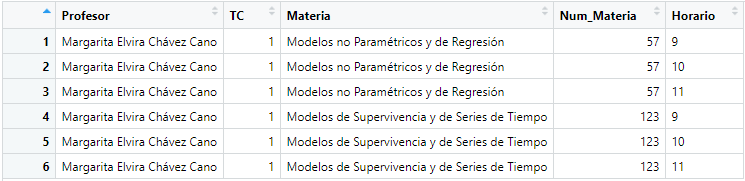
\includegraphics[width=\textwidth]{mat_1_solicitud_Margarita} %scale = 0.8
\caption[\textit{Ejemplo de matriz de solicitudes de un profesor}]{\textit{Ejemplo de matriz de solicitudes de un profesor: Se observa un ejemplo de la matriz mat\_1\_solicitud para un profesor de tiempo completo.}}\label{mat_1_solicitud_Margarita}
\end{figure}

El proceso se repite para cada uno de los profesores en la matriz \textit{mat\_nom\_prof\_total} obtenida en la Sección \ref{nomProfesores}. La matriz formada con las solicitudes de todos los profesores la llamamos \textit{mat\_solicitudes}. A ella le quitamos los renglones repetidos para poder simular adecuadamente los esqueletos.
